% Chapter Template

\chapter{Localization of Humanoid Robot} % Main chapter title

\label{Chapter4} % Change X to a consecutive number; for referencing this chapter elsewhere, use \ref{ChapterX}

\lhead{Chapter 4. \emph{Localization of Humanoid Robot}} 
		The localization of humanoid robots is a challenging issue, due to rough odometry estimation, noisy onboard sensing, and the swaying motion caused by walking\cite{Cervera2012}. 
		 
		As a prelimnary assumption, the link of the robot are considered \emph{rigid bodies} in which distance between any two given points on it remains constant in time regardless of external forces exerted on it. Rigid body transformation forms the basic components in the pose estimation framework. In the $3D$ operational space represented by the vector space $\Re^3$, a rigid body is represented by \emph{6 degrees of freedom (DOF)}, 3 for the position along each of the coordinate axes (cartesian coordinates) $P = [p_x,p_y,p_z]^{\text{T}}$ and 3 for the orientation $R$. There are different representation for the orientation of the rigid body. They are rotation matrices, euler angles, RPY (roll,pitch,yaw) angles, quaternions. A detailed introduction about rigid body mechanics and various representation of pose of a rigid body can be found in the book by Khalil\cite{Khalil2002}.
		
		For most of the humanoid robots the reference frame will be fixed to the torso as is the case for the Nao. So the basic idea is to track the torso of the Nao or any other position with the known transformation from the torso. In this section different techniques that could be effectively used for localization and tracking of the humanoid robot are presented.
\section{Artificial Marker based approaches}
	The advancements in the field of augmented reality led to the development of efficient tracking of object poses by employing fiducial markers. Tracking rectangular fiducial markers can be interesting if we could embed those markers on the humanoid robot. This is one of the simplest and cheapest solution in terms of the computational power as it uses simple image processing algorithms. ARToolKit\cite{Kato1999} implements video tracking libraries which can calculate the real camera position and orientation relative to physical markers in real time. Before camera-based 6DOF tracking can be performed, the camera must be calibrated once as a pre-processing step. The perspective projection and the camera distortion parameters obtained during this step will be used later during the tracking initialization phase. During the tracking, as a first step ARToolKit performs a very simple edge detection by thresholding the complete image with a constant value, followed by a search for quadrangles. Resulting areas being either too large or too small are immediately rejected. Next the interior areas of the remaining quadrangles are normalized using a perspective transformation. The resulting sub-images are then checked against the set of known patterns. When a pattern is detected, ARToolKit uses the marker’s edges for a first, coarse pose detection. In the next step the rotation part of the estimated pose is refined iteratively using matrix fitting. The resulting pose matrix defines a transformation from the camera plane to a local coordinate system in the centre of the marker. ARToolKit can combine several co-planar markers into a multi-marker set. From an application point of view this multi-marker set is treated as a single marker and can be tracked as long as one or more markers of this set are visible. Multi-marker tracking increases the computational load but results in considerably more accurate and robust tracking. ARToolKit also gives the possibility for user-defined markers and the libraries could be trained to track those markers in real time.
\begin{figure}[H]
\centering
\includegraphics[width=1\textwidth]{assets/artoolkit.eps}
\caption[Marker tracking using ARToolKit]{Marker tracking using ARToolKit. {Adapted from \cite{Kato1999}}}
\label{fig:artoolkit}
\end{figure}
\section{Point Cloud based approaches}
\label{ssec:pcl}
	The Point Cloud Library (PCL)\cite{RusuPCL11} which is one of the most widely used 3D perception software library, has collection of state-of-the-art algorithms and tools to process 3-D data. The library is open source and licensed under Berkeley Software Distribution (BSD) terms and, therefore, free to use for everyone. Due to this fact the community has ease of access to powerful ready to use algorithms. In this section, different pose recognition techniques using the point clouds are presented.
\subsection{PCL Pose estimation Pipeline}
	Point cloud library provides an excellent infrastructure for the object recognition and 6DOF pose estimation pipeline by offering a wide variety of robust local and global features. A list of features available is presented in \cite{PCL2012}. Object recognition based on global/local features almost share the same flow of operations. A glimpse of the pipeline is shown in Figure~\ref{fig:pcl_pipeline}.
\begin{figure}[H]
\centering
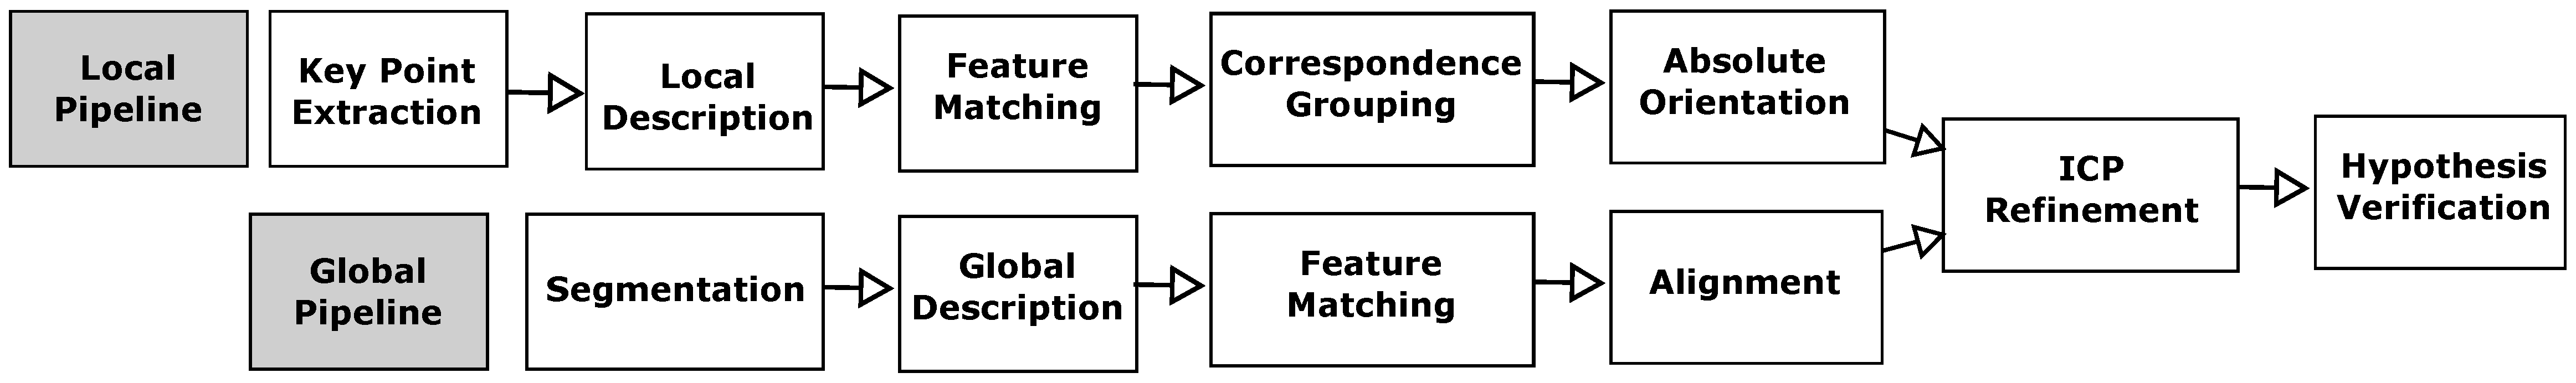
\includegraphics[width=1\textwidth]{assets/pcl_pipeline.eps}
\caption[PCL local and global 3D Pipelines]{PCL local and global 3D Pipelines. {Adapted from \cite{PCL2012}}}
\label{fig:pcl_pipeline}
\end{figure}
Before the PCL system being able to detect the pose of the object, the system has to be trained with the point clouds of the meshes generated by a virtual depth camera. The 3D features of the model are computed and stored to be used during the recognition phase. 
	The first step in the recognition based on \emph{local descriptors} is \emph{key-point extraction} which detect repeatable and distinct key points from the scene data. After this step, they are associated to a \emph{local description} defined over a local support for determining the subset of neighbouring points around the key point. Once descriptor are computed for the current scene and each model in the library, \emph{matching} will be performed to yield point-to-point correspondences. This is followed by an additional stage called \emph{correspondence grouping} during which correspondence which are not geometrically consistent are discarded. However this step does not guarantee that all remaining correspondences are consistent with unique 6-DOF pose. To this purpose Random Sampling Consensus(RANSAC) is used to remove the outliers. Following this, a least square optimization is performed to obtain the rotation and the translation from exact point correspondences.
	
	For recognition based on global descriptors, the first step involves a \emph{segmentation} of the scene to extract the objects in it based on the extraction of a dominant scene plane and euclidean clustering step. During the \emph{description and matching} steps, the shape and geometry of each objects in the scene are described using appropriate global descriptor and represented by one or more histograms. The histogram \emph{matching} is done to those obtained during training stage to retrieve $N$-nearest neighbors using \emph{FLANN (Fast Library for Approximate nearest neighbors)}. An aliging step following this will give a 5-DoF pose since the global descriptors are invariant to roll axis rotation. This rotation could be achieved using \emph{camera roll histogram}.Both the global and local pipelines can undergo an optional \emph{post processing} step by applying Iterated Closest Point (ICP) in order to refine estimated 6-DoF pose. The following step referred to as \emph{hypotheses verification} which aims at reducing false positives(FPs).
\subsection{PCL Tracking pipeline}
	Apart from the object recognition and pose estimation pipeline, PCL\cite{RUeda2012} provides a comprehensive algorithmic base for the estimation of 3D object poses using Monte Carlo sampling techniques and for calculating the likelihood using combined weighted metrics for hyperdimensional spaces including cartesian data, colors, and surface normals. PCL also has non-probabilistic tracking algorithms like Pyramidal Kanade Lucas Tomasi(KLT) Tracker in its tracking module. The KLT tracker operates on organized 3D keypoints with color/intensity information. It is an affine tracker that iteratively computes the optical flow to find the best guess for a point $p$ at time $t$ given its location at $t-1$. A list of probabilistic tracking algorithms implemented in PCL is presented in Section~\ref{sssec:prob_solutions} for the purpose of being coherent.
\section{Probabilistic Approaches}
\label{ssec:prob_approaches}
	Probabilistic localization algorithms are variants of the Bayes filter\cite{Thrun2005}. The pose of the robot is represented in a probabilistic manner called the \emph{belief}: ($bel(x_t)$) which is a posterior distribution over the state space. The basic principle behind Bayes filter is that the belief $bel(x_t)$ at time $t$ is calculated from the belief $bel(x_{t-1})$ at time $t-1$ along with the most recent control $u_t$ and the most recent measurement $z_t$. It involves two basic steps: \emph{Control update step} during which the $\overline{bel(x_t)}$ is computed based on the prior assigned to $x_{t-1}$ and the probability that control $u_t$ induces a transition from $x_{t-1}$ to $x_t$, \emph{Measurement update step} during which the hypothetical posterior $\overline{bel(x_t)}$ is multiplied with the probability of seeing an observation $z_t$ given this $x_t$. The recursive computation of belief state can thus be given by
	\begin{align*}
	\text{Control update step:}\quad \overline{bel(x_t)} &= \int p(x_t\vert u_t,x_{t-1})\cdot bel(x_{t-1}) dx \\
	\text{Measurement update step:}\quad {bel(x_t)} &= \eta\cdot p(z_t\vert x_{t})\cdot \overline{bel(x_t)}
	\end{align*}
	where $\eta$ is the normalization factor.
	The straightforward application of Bayes filters to the localization problem is called Markov localization. Markov localization makes use of the \emph{Markov assumption} (The Markov
assumption postulates that past and future data are independent if one knows the current
state {$x_t$). Extended Kalman Filter(EKF) based localization is one of the initial developments to be used in non-linear state models. However they suffered problems of uni-modal distribution(gaussian) assumption and failing to solve global localization problem. In the following section, a class of non-parametric localization approach is presented. 
\subsection{Particle Filter}
\label{ssec:particlefilter}
	The particle filter\cite{Thrun2005} is an alternative non parametric implementation of Bayes filter. The key idea of the particle filter is to represent the posterior $bel(x_t)$ by a set of samples drawn from the distribution. Such a representation is approximate, but it is nonparametric, and therefore can represent a much broader space of distributions than, for example, Gaussians. The important components of a particle filter are\\
\begin{tabular}{r l}
\centering
  (Control input,Measurement) & $(u_t,z_t)$ \\ 
  Sample of Posterior distribution (particles) & $X_t := {x_t}^{[1]},{x_t}^{[2]},\cdots,{x_t}^{[M]}$ \\
  (Posterior PDF,Likelihood function) & $(p(X_t\vert z_{1:t}),p(z_t \vert {x_t}^{[m]})$ \\
  Importance Factor of $m^{th}$ particle & ${w_t}^{[m]}$ \\
\end{tabular}
	
	Each particle ${x_t}^{[m]}$ (with $1 \leq m \leq M$) is the concrete instantiation of the state at time $t$, that a hypothesis as to what the true world state may be at $t$. Here $M$ denotes the number of particles in the set $X_t$. The basic intuition behind the particle filter is to approximate the belief $bel(x_t)$ by the set of particles $X_t$ and as a consequence denser a subregion of the state space is populated by samples, the more likely the true state falls in the region.The current state is given by the weighted particle mean 
\begin{equation}
E(X_t) = \sum_{m=1}^{M} {w_t}^{[m]}\cdot {x_t}^{[m]}
\end{equation}
The basic algorithm of particle filter is shown in \ref{alg:particlefilter}.\\ 
\begin{algorithm}
\KwData{$X_{t-1}$, $u_t$, $z_t$}
\KwResult{$X_t$}
Init: {$\tilde{X_t}$ = $X_t$ = $\emptyset$ } \;
 \For{$m$ = $1$ to $M$} { 
   sample ${x_t}^{[m]} \approx p(x_t \vert u_t,{x_{t-1}}^{[m]}) $ //Hypothetical state computation \;
   ${w_t}^{[m]} = p(z_t \vert {x_t}^{[m]} )$ //Importance factor computation\;
   $\tilde{X_t} = \tilde{X_t} + ({x_t}^{[m]},{w_t}^{[m]})$ \;
 }
 \For{$m$ = $1$ to $M$} { 
   draw $i$ with probability $\varpropto$ ${w_t}^{[i]}$ //Importance re-sampling\;
   add ${x_t}^{[i]}$ to $X_t$ \;
 }
 return $X_t$
 \caption{Basic algorithm of Particle Filter}
 \label{alg:particlefilter}
\end{algorithm}
\subsection{Monte Carlo Localization}
\label{ssec:montecarlo}
	Monte-carlo localization (MCL)\cite{Fox99montecarlo} is a version of Markov localization, a family of probabilistic approaches that has been successfully applied to localization problems and it has become one of the most popular localization algorithms in robotics. MCL uses fast sampling techniques to represent the belief and it introduces probabilistic motion and perceptual models into the particle filter framework. Hence it uses the same formalism described in \ref{ssec:particlefilter}.\\  	
\begin{algorithm}
\KwData{$X_{t-1}$, $u_t$, $z_t$}
\KwResult{$X_t$}
Init: {$\tilde{X_t}$ = $X_t$ = $\emptyset$ } \;
 \For{$m$ = $1$ to $M$} { 
   ${x_t}^{[m]} = \text{sample\_motion\_model}(u_t,{x_{t-1}}^{[m]})$ //Hypothetical state computation\;
   ${w_t}^{[m]} = \text{measurement\_model}(z_t,{x_t}^{[m]},m)$ //Importance factor computation \; 
   $\tilde{X_t} = \tilde{X_t} + ({x_t}^{[m]},{w_t}^{[m]})$ \;
 }
 \For{$m$ = $1$ to $M$} { 
   draw $i$ with probability $\varpropto$ ${w_t}^{[i]}$ //Importance re-sampling\;
   add ${x_t}^{[i]}$ to $X_t$ \;
 }
 return $X_t$
 \caption{Monte Carlo Localization}
 \label{alg:montecarlo}
\end{algorithm}

	The efficiency of particle filters lies in the way they place computational resources. By sampling in proportion to likelihood, particle filters focus the computational resources on regions with high likelihood, where good approximations are most important. The time complexity of one update of the particle filter algorithm is linear in the number of samples needed for the estimation. The Kullback-Leibler Distance(KLD) adaptive sampling technique proposed in \cite{Fox03adaptingthe} presents an approach to adapt the number of samples over time. The key idea is at each iteration of the particle filter, the number of samples are determined such that, with probability $1-\delta$, the error between the true posterior and the sample-based approximation (maximum likelihood estimate- MLE) is less than $\epsilon$. The distance between the MLE and the true distribution is measured by a non-negative Kullback-Leibler distance which for two distributions $p$ and $q$ is given by
\begin{equation}
K(p,q) = \sum_{x} p(x)log{\frac{p(x)}{q(x)}}
\end{equation}

\subsection{Existing Solutions}
\label{sssec:prob_solutions}
	\par The Point cloud library\cite{RUeda2012} introduced in Section~\ref{ssec:pcl} implements ready to use probabilistic tracking algorithms like: the most basic particle filter tracker(\emph{ParticleFilterTracker}), particle filter using OpenMP support(\emph{ParticleFilterOMPTracker}), KLD-adaptive sampling particle filter( \emph{KLDAdaptiveParticleFilterTracker}) and KLD adaptive sampling with OpenMP support ( \emph{KLDAdaptiveParticleFilterOMPTracker}). This could be readily used to track an object of know geometry and this information has to be fed to the PCL through a point cloud mesh of the object.
	
	Studies on robot localization, obstacle mapping, and path planning in multilevel 3D environments by equipping Nao with a consumer-level depth camera has been reported in \cite{Maier2012}. This study provides real-time solution while maintaining a 3D environment representation and estimating the robot’s pose in 6D. The 3D environment model in form of an octree based representation containing the static parts of the environment is used. In this representation, the robot estimates its pose using MCL based on acquired depth data. Given the estimated 6D pose of the humanoid and a sequence of depth images, this approach continuously builds a local 3D representation of the current state of the environment containing also non-static obstacles. This learned octree-based representation is then used for real-time planning of collision-free paths. For robust localization while walking, it combines 3D range data from the depth camera located on top of the head, altitude data provided by an inertial measurement unit (IMU) in the chest and odometry data.
	
	While \cite{Maier2012} presented an approach wherein a depth camera is fixed to the humanoid robot, in \cite{Cervera2012} localization and motion planning in smart home environment have been proposed. In this study an external depth camera is used for 6D pose estimation and tracking, which is very close to the scenario of this thesis. Once again MCL technique is used for the pose estimation of the torso of the humanoid robot and this information is used for the closed loop navigation control. For the localization, this study used  \emph{KLDAdaptiveParticleFilterOMPTracker} available in Point cloud library. For the purpose of navigation, this study determined the pose error on the plane of walking using the knowledge of estimated pose and the desired pose. The linear velocity of the robot is calculated from the pose error using a proportional gain. The angular velocity is determined adaptively depending on the distance to the target. The localization results of this study proved to be robust compared to the odometry data. However this study did not take into account of collision free navigation planning. 
	
	In \cite{choi13_rgb_d_objec_track} a robust particle filter parallelized on a GPU that can track a known 3D object model over a sequence of RGB-D images is proposed. This method proposes to render the 3D object model to be used in the likelihood function so that the object could be tracked inspite of significant pose variations. Unlike PCL object tracking algorithm\cite{RusuPCL11} which maintains only one reference point cloud, this approach uses multiple viewports rendered in GPU with different poses and each particle searches the closest rendering from the viewports and likelihood evaluation is performed by transforming the closest rendered result with the current particle state. Each particle is defined as 6D vector consisting of position and orientation of the object. For the likelihood evaluation, this work exploits the RGB-D data and utilizes the position, normal and color information of the points. Through a set of extensive experiments with both synthetic and real RGB-D sequences, this approach has been proved to be faster and also accurate than the PCL tracking.
	
%For the likelihood evaluation, this work exploits the RGB-D data and utilizes the measurement vector of the $i^{th}$ point at $t^{th}$ instant $z_t^{[i]} \in \Re^9$ defined as follows
%\begin{equation}
%z_t^{[i]} = ({p_t^{[i]}}^{\text{T}},{n_t^{[i]}}^{\text{T}},{c_t^{[i]}}^{\text{T}})^{\text{T}}
%\end{equation}
%where ${p_t^{[i]}}^{\text{T}} \in \Re^3$:Position, ${n_t^{[i]}}^{\text{T}} \in \Re^3$:Normal, ${c_t^{[i]}}^{\text{T}} \in \Re^3$:Color. Additionally the operators to access Position, Normal and Color given the ${z_t}^{[i]}$ are definded as $pt({z_t}^{[i]})=({p_t^{[i]}}^{\text{T}} 1)^{\text{T}} \in \Re^4$, $n({z_t}^{[i]})=({n_t^{[i]}}^{\text{T}} 1)^{\text{T}} \in \Re^4$ and $c({z_t}^{[i]})=(c_t^{[i]}) \in \Re^3$ respectively. 
%From the current pose hypothesis ${x_t}^{[m]}$ and the rendered object model $M_t$, the likelihood of the scene $z_t$ is defined as 
%\begin{equation}
%p(z_t\vert {x_t}^{[m]},M_t) = \prod_{(i,j)\in A} p({z_t}^{[i]}\vert {x_t}^{[m]},{m_t}^{[j]})
%\end{equation}
%where $A=\lbrace (i,j)\vert proj(pt({z_t}^{[i]})) = proj(x_t^{m}.pt({m_t}^{[j]})) \rbrace$ is the set of point associations between the scene $z_t$ and the object model $M_t$ and ${z_t}^{[i]},{m_t}^{[j]} \in \Re^9$ are corresponding points in the scene and model respectively. The operator $proj(.)$ computes the 2D image coordinates from the 3D homogenous point coordinates by projecting the point with the known camera intrinsic parameters $K \in \Re^{3\times 3}$. The likelihood of each association $(i,j)$ is then defined by 
%\begin{align*}
%p({z_t}^{[i]}\vert {x_t}^{[m]},{m_t}^{[j]}) &= \text{exp}^{-\lambda_e.d_e(pt({z_t}^{[i]}),x_t^{m}.pt({m_t}^{[j]}))}\cdot \\
%										   &\quad\ \text{exp}^{-\lambda_n.d_n(n({z_t}^{[i]}),x_t^{m}.n({m_t}^{[j]}))}\cdot \\								   &\quad\ \text{exp}^{-\lambda_c.d_c(c({z_t}^{[i]}),x_t^{m}.c({m_t}^{[j]}))}
%\end{align*}
%where $d_e(p_1,p_2)$, $d_n(n_1,n_2)$ and $d_c(c_1,c_2)$ are euclidean, normal and color distances.
%% as shown below
%%\begin{align*}
%%d_e(p_1,p_2) &= \begin{cases}
%%\Vert p_1 - p_2 \Vert &\quad\quad \text{ if } \Vert p_1 - p_2 \Vert \leq \text{ threshold} \\
%%1					  &\quad\quad \text{ otherwise } \\
%%\end{cases}\\
%%d_n(n_1,n_2) &= \frac{cos^{-1}(n_1^{\text{T}}n_2-1)}{\pi} \\
%%d_c(c_1,c_2) &= \Vert c_1 - c_2 \Vert
%%\end{align*}
%%and 
%$(\lambda_e,\lambda_n,\lambda_c)$ are the parameters that determine the sensitivity of the distances to the likelihood. 




%Since the normals $(n_1,n_2)$ are represented as homogenous coordinates, $1$ has to be subtracted from their inner product. As far as $d_c$ is concerned, HSV color space is considered for $(c_1,c_2)$ due to the invariance to illumination changes.

%\subsubsection{Pose detection using Particle Filter and RGB-D data}
%\label{ssec:particlegpu}
% In \cite{choi13_rgb_d_objec_track}, a robust particle filter parallelized on a GPU that can track a known 3D object model $M_t$ over a sequence of RGB-D images is proposed. This method proposes to render the 3D object model to be used in the likelihood function so that the object could be tracked inspite of significant pose variations. The key features of the study include
%
%\begin{itemize}
%\item Unlike traditional methods which employed 2D edges, intensity differences to calculate the importance weight of the particles, this approach uses both photometric(colors) and geometric features (3D points and surface normals) available from RGB-D images and OpenGL rendering.
%\item It uses the framebuffer object extension (FBO) in OpenGL and the CUDA OpenGL interoperability to reduce the mapping time of the rendering result to CUDA’s memory space.
%\item Unlike PCL object tracking algorithm\cite{RusuPCL11} which maintains only one reference point cloud, this approach uses multiple viewports rendered in GPU with different poses and each particle searches the closest rendering from the viewports and likelihood evaluation is performed by transforming the closest rendered result with the current particle state.
%\end{itemize}
%
%Each particle $x_t$ is a 6D vector consisting of Position and Orientation $x_t: (P_t,R_t)$ of the object. As described in the previous section~\ref{ssec:particlefilter}, the pose of the object is given by the weighted particle mean. However when we estimate the mean, it should give a valid rotation $R_t \in SO(3)$ as the arithmetic mean $\tilde{R_t}=\frac{1}{M}\sum_{m=1}^{M} {R_t}^{[m]}$ is not usually on the $SO(3)$ group. In order to overcome this problem the desired mean is calculated via the orthogonal projection of the arithmetic mean as
%
%\begin{equation}
%R_t = \begin{cases}
%VU^{\text{T}}  \quad\quad when \det(\tilde{R}^{\text{T}}) > 0 \\
%VHU^{\text{T}} \quad\quad otherwise
%\end{cases}
%\end{equation}
%
%where $U$ and $V$ are estimated via the singular value decomposition of $\tilde{R}^{\text{T}}$ (\textit{i.e} $\tilde{R}^{\text{T}}$ = $U\Sigma V^{\text{T}}$) and $H=diag[1,1,-1]$.
%
%For the likelihood evaluation, this work exploits the RGB-D data and utilizes the measurement vector of the $i^{th}$point at $t^{th}$ instant $z_t^{[i]} \in \Re^9$ defined as follows
%
%\begin{equation}
%z_t^{[i]} = ({p_t^{[i]}}^{\text{T}},{n_t^{[i]}}^{\text{T}},{c_t^{[i]}}^{\text{T}})^{\text{T}}
%\end{equation}
%
%where ${p_t^{[i]}}^{\text{T}} \in \Re^3$:Position, ${n_t^{[i]}}^{\text{T}} \in \Re^3$:Normal, ${c_t^{[i]}}^{\text{T}} \in \Re^3$:Color. Additionally the operators to access Position, Normal and Color given the ${z_t}^{[i]}$ are definded as $pt({z_t}^{[i]})=({p_t^{[i]}}^{\text{T}} 1)^{\text{T}} \in \Re^4$, $n({z_t}^{[i]})=({n_t^{[i]}}^{\text{T}} 1)^{\text{T}} \in \Re^4$ and $c({z_t}^{[i]})=(c_t^{[i]}) \in \Re^3$ respectively. 
%
%From the current pose hypothesis ${x_t}^{[m]}$ and the rendered object model $M_t$, the likelihood of the scene $z_t$ is defined as 
%
%\begin{equation}
%p(z_t\vert {x_t}^{[m]},M_t) = \prod_{(i,j)\in A} p({z_t}^{[i]}\vert {x_t}^{[m]},{m_t}^{[j]})
%\end{equation}
%
%where $A=\lbrace (i,j)\vert proj(pt({z_t}^{[i]})) = proj(x_t^{m}.pt({m_t}^{[j]})) \rbrace$ is the set of point associations between the scene $z_t$ and the object model $M_t$ and ${z_t}^{[i]},{m_t}^{[j]} \in \Re^9$ are corresponding points in the scene and model respectively. The operator $proj(.)$ computes the 2D image coordinates from the 3D homogenous point coordinates by projecting the point with the known camera intrinsic parameters $K \in \Re^{3\times 3}$. The likelihood of each association $(i,j)$ is then defined by 
%
%%\begin{equation}
%\begin{align*}
%p({z_t}^{[i]}\vert {x_t}^{[m]},{m_t}^{[j]}) &= \text{exp}^{-\lambda_e.d_e(pt({z_t}^{[i]}),x_t^{m}.pt({m_t}^{[j]}))}\cdot \\
%										   &\quad\ \text{exp}^{-\lambda_n.d_n(n({z_t}^{[i]}),x_t^{m}.n({m_t}^{[j]}))}\cdot \\								   &\quad\ \text{exp}^{-\lambda_c.d_c(c({z_t}^{[i]}),x_t^{m}.c({m_t}^{[j]}))}
%\end{align*}
%
%where $d_e(p_1,p_2)$, $d_n(n_1,n_2)$ and $d_c(c_1,c_2)$ are euclidean, normal and color distances as shown below
%
%\begin{align*}
%d_e(p_1,p_2) &= \begin{cases}
%\Vert p_1 - p_2 \Vert &\quad\quad \text{ if } \Vert p_1 - p_2 \Vert \leq \text{ threshold} \\
%1					  &\quad\quad \text{ otherwise } \\
%\end{cases}\\
%d_n(n_1,n_2) &= \frac{cos^{-1}(n_1^{\text{T}}n_2-1)}{\pi} \\
%d_c(c_1,c_2) &= \Vert c_1 - c_2 \Vert
%\end{align*}
%
%and $(\lambda_e,\lambda_n,\lambda_c)$ are the parameters that determine the sensitivity of the distances to the likelihood. Since the normals $(n_1,n_2)$ are represented as homogenous coordinates, $1$ has to be subtracted from their inner product. As far as $d_c$ is concerned, HSV color space is considered for $(c_1,c_2)$ due to the invariance to illumination changes.